\documentclass[PianoDiProgetto.tex]{subfiles}
%TODO sistemare tabelle e immagini
\begin{document}
\chapter{Suddivisione risorse e preventivo}
\section{Analisi}
\subsection{Prospetto Orario}
Nel periodo di Analisi la distribuzione oraria è la seguente:
\begin{center}

\begin{table}[htbp]
	\centering
	\renewcommand\arraystretch{1.5}
	\begin{tabularx}{\textwidth}{p{4cm}|p{1cm}|p{1cm}|p{1cm}|p{1cm}|p{1cm}|p{1cm}|p{2cm}}
		\hline
		\textbf{Nome} & \textbf{Re} & \textbf{Ad} & \textbf{An} & \textbf{Pj} & \textbf{Pr} & \textbf{Ve} & \textbf{Totale} \\
		\hline
		\Davide & \ & 8 & 8 & \ & \ & 6 & \textbf{22} \\
		\hline
		\Elena & 4 & 4 & 14 & \ & \ & 0 & \textbf{22} \\
		\hline
		\Gianluca & 4 & 0 & 12 & \ & \ & 6 & \textbf{22} \\
		\hline
		\Mirco & \ & 4 & 14 & \ & \ & 4 & \textbf{22} \\
		\hline
		\Parwinder & 8 & \ & 14 & \ & \ & 6 & \textbf{22} \\
		\hline
		\Riccardo & 4 & \ & 12 & \ & \ & 6 & \textbf{22} \\
		\hline
		\Valentina & 4 & \ & 10 & \ & \ & 8 & \textbf{22} \\
		\hline
	\end{tabularx}
	\caption{Distribuzione oraria del periodo di Analisi}
	\label{my-label}
\end{table} 
\newpage	
\end{center}
Il seguente grafico dà una rappresentazione visiva della suddivisione oraria:
\begin{figure}[h]
	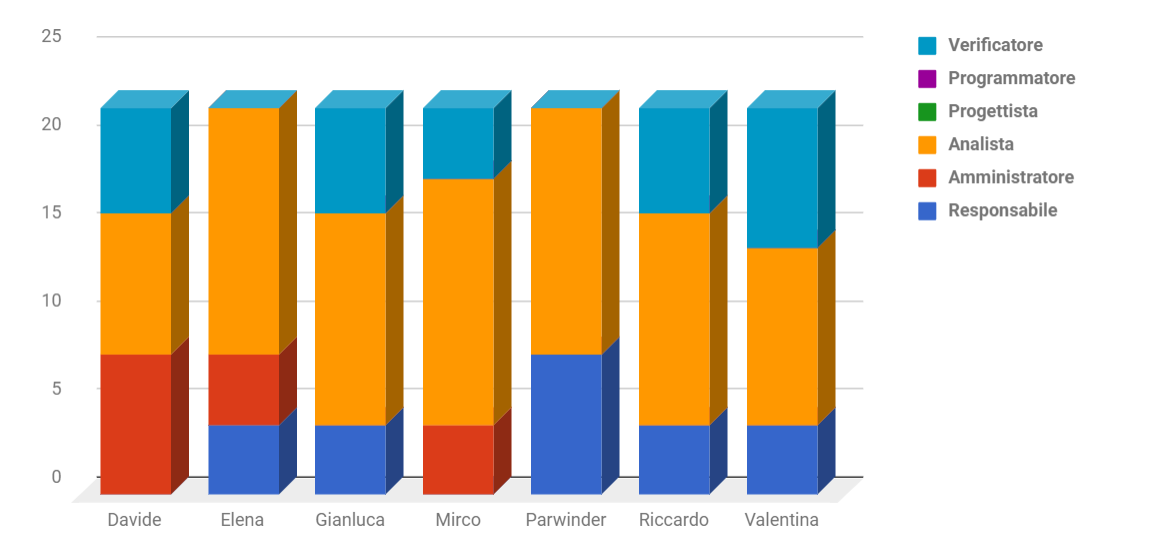
\includegraphics[width=14.5cm]{images/prospettoOrario/analisi.png}
	\label{fig:foo}
	\caption{Grafico suddivisione oraria del periodo di Analisi}
\end{figure} 

\subsection{Prospetto Economico}
Nel periodo di Analisi la distribuzione delle ore tra i differenti ruoli è la seguente:\\
\begin{table}[htbp]
	\centering
	\renewcommand\arraystretch{1.5}
	\begin{tabularx}{\textwidth}{p{5cm}|p{4cm}|p{4cm}}
		\hline
		\textbf{Ruolo} & \textbf{Ore} & \textbf{Costo in \euro} \\
		\hline
		Responsabile & 24 & 720,00 \\
		\hline
		Amministratore & 16 & 320,00 \\
		\hline
		Analista & 84 & 2.100,00 \\
		\hline
		Progettista & \ & \ \\
		\hline
		Programmatore & \ & \ \\
		\hline
		Verificatore & 30 & 450,00 \\
		\hline
		\textbf{Totale} & \textbf{154} & \textbf{3590,00}\\
		\hline
	\end{tabularx}
	\caption{Prospetto economico del periodo di Analisi}
	\label{my-label}
\end{table} \newpage
Il seguente grafico dà una rappresentazione visiva della distribuzione dei ruoli:
\begin{figure}[h]
	\centering
	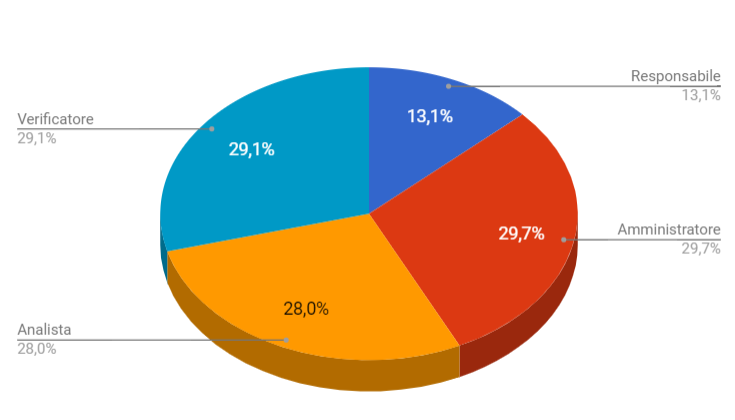
\includegraphics[width=10.5cm]{images/prospettoEconomico/analisi.png}
	\label{fig:foo}
	\caption{Grafico suddivisione dei ruoli del periodo di Analisi}
\end{figure} 
\section{Consolidamento dei requisiti}
\subsection{Prospetto Orario}
Nel periodo di Consolidamento dei requisiti la distribuzione oraria è la seguente:
\begin{center}

\begin{table}[htbp]
	\centering
	\renewcommand\arraystretch{1.5}
	\begin{tabularx}{\textwidth}{p{4cm}|p{1cm}|p{1cm}|p{1cm}|p{1cm}|p{1cm}|p{1cm}|p{2cm}}
		\hline
		\textbf{Nome} & \textbf{Re} & \textbf{Ad} & \textbf{An} & \textbf{Pj} & \textbf{Pr} & \textbf{Ve} & \textbf{Totale} \\
		\hline
		\Davide & \ & 3 & 3 & \ & \ & \ & \textbf{6} \\
		\hline
		\Elena & 4 & \ & 2 & \ & \ & \ & \textbf{6} \\
		\hline
		\Gianluca & \ & \ & 6 & \ & \ & \ & \textbf{6} \\
		\hline
		\Mirco & \ & \ & 6 & \ & \ & \ & \textbf{6} \\
		\hline
		\Parwinder & \ & 4 & \ & \ & \ & 2 & \textbf{6} \\
		\hline
		\Riccardo & \ & 2 & \ & \ & \ & 4 & \textbf{6} \\
		\hline
		\Valentina & \ & \ & \ & \ & \ & 6 & \textbf{6} \\
		\hline
	\end{tabularx}
	\caption{Distribuzione oraria del periodo di Consolidamento dei requisiti}
	\label{my-label}
\end{table}
\end{center}
\newpage
Il seguente grafico dà una rappresentazione visiva della suddivisione oraria:

\begin{figure}[h]
	\centering
	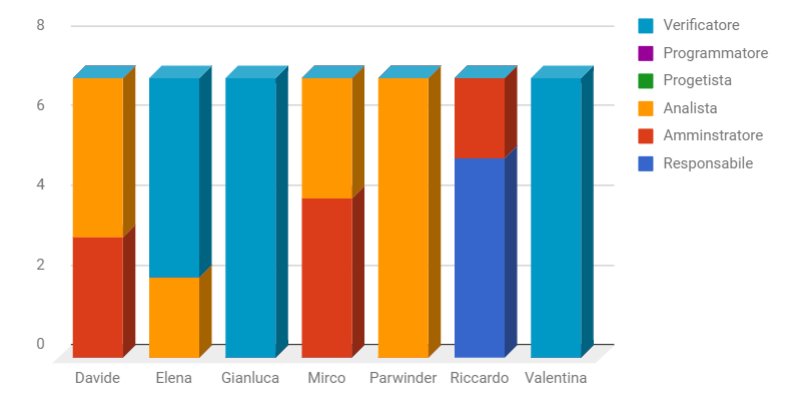
\includegraphics[width=14.5cm]{images/prospettoOrario/consolidamento.png}
	\label{fig:foo}
	\caption{Grafico suddivisione oraria del periodo di Consolidamento dei requisiti}
\end{figure} 
\subsection{Prospetto Economico}
Nel periodo di Analisi la distribuzione delle ore tra i differenti ruoli è la seguente:
\begin{center}
\begin{table}[htbp]
	\centering
	\renewcommand\arraystretch{1.5}
	\begin{tabularx}{\textwidth}{p{5cm}|p{4cm}|p{4cm}}
		\hline
		\textbf{Ruolo} & \textbf{Ore} & \textbf{Costo in \euro} \\
		\hline
		Responsabile & 4 & 120,00 \\
		\hline
		Amministratore & 9 & 180,00 \\
		\hline
		Analista & 17 & 425,00 \\
		\hline
		Progettista & \ & \ \\
		\hline
		Programmatore & \ & \ \\
		\hline
		Verificatore & 12 & 180,00 \\
		\hline
		\textbf{Totale} & \textbf{42} & \textbf{905,00}\\
		\hline
	\end{tabularx}
\caption{Prospetto economico del periodo di Consolidamento dei requisiti}
\label{my-label}
\end{table} 
\end{center}
\clearpage
Il seguente grafico dà una rappresentazione visiva della distribuzione dei ruoli:
\begin{figure}[h]
	\centering
	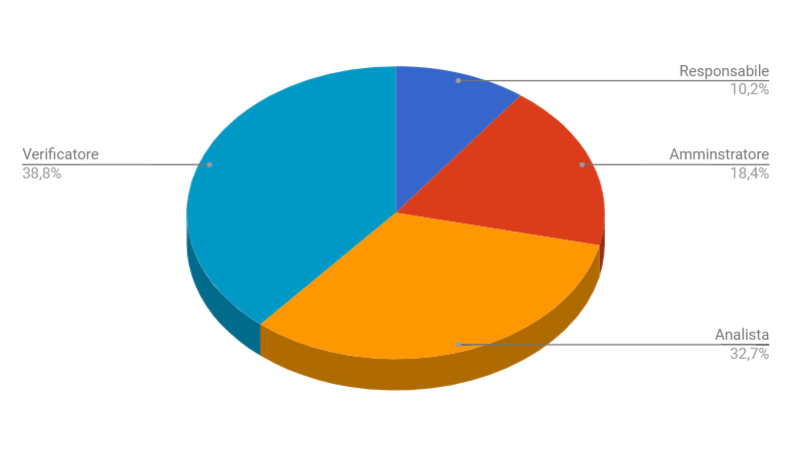
\includegraphics[width=10.5cm]{images/prospettoEconomico/consolidamento.png}
	\label{fig:foo}
	\caption{Grafico suddivisione dei ruoli del periodo di Consolidamento dei requisiti}
\end{figure} 
\clearpage
\section{Progettazione architetturale}
\subsection{Prospetto Orario}
Nel periodo di Progettazione architetturale la distribuzione oraria è la seguente:
\begin{center}
\begin{table}[htbp]
	\centering
	\renewcommand\arraystretch{1.5}
	\begin{tabularx}{\textwidth}{p{4cm}|p{1cm}|p{1cm}|p{1cm}|p{1cm}|p{1cm}|p{1cm}|p{2cm}}
		\hline
		\textbf{Nome} & \textbf{Re} & \textbf{Ad} & \textbf{An} & \textbf{Pj} & \textbf{Pr} & \textbf{Ve} & \textbf{Totale} \\
		\hline
		\Davide & 4 & \ & 10 & 12 & \ & 4 & \textbf{30} \\
		\hline
		\Elena & \ & \ & \ & 20 & \ & 10 & \textbf{30} \\
		\hline
		\Gianluca & \ & 5 & \ & 15 & \ & 10 & \textbf{30} \\
		\hline
		\Mirco & 4 & \ & \ & 20 & \ & 6 & \textbf{30} \\
		\hline
		\Parwinder & \ & \ & \ & 15 & \ & 15 & \textbf{30} \\
		\hline
		\Riccardo & \ & 5 & \ & 20 & \ & 5 & \textbf{30} \\
		\hline
		\Valentina & 2 & \ & 10 & 10 & \ & 8 & \textbf{30} \\
		\hline
	\end{tabularx}
	\caption{Distribuzione oraria del periodo di Progettazione architetturale}
	\label{my-label}
\end{table}
\end{center}
Il seguente grafico dà una rappresentazione visiva della suddivisione oraria:
\begin{figure}[h]
	\centering
	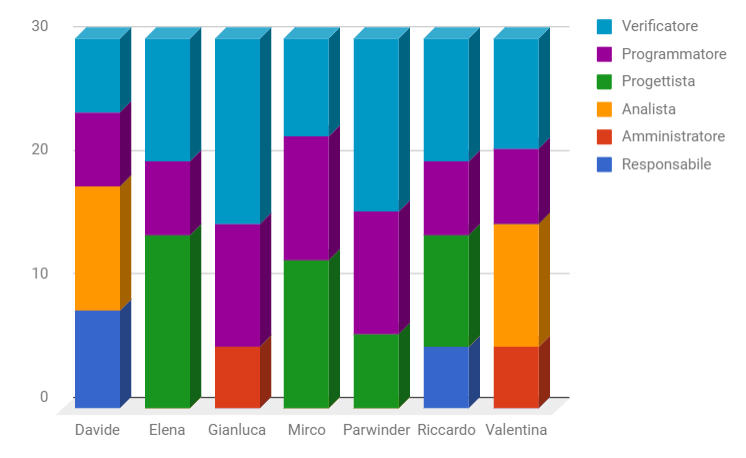
\includegraphics[width=10.5cm]{images/prospettoOrario/progArch.png}
	\label{fig:foo}
	\caption{Grafico suddivisione oraria del periodo di Progettazione architetturale}
\end{figure} 
\newpage
\subsection{Prospetto Economico}
Nel periodo di Progettazione architetturale la distribuzione delle ore tra i differenti ruoli è la seguente:
\begin{center}
\begin{table}[htbp]
	\centering
	\renewcommand\arraystretch{1.5}
	\begin{tabularx}{\textwidth}{p{5cm}|p{4cm}|p{4cm}}
		\hline
		\textbf{Ruolo} & \textbf{Ore} & \textbf{Costo in \euro} \\
		\hline
		Responsabile & 10 & 300,00 \\
		\hline
		Amministratore & 10 & 200,00 \\
		\hline
		Analista & 20 & 500,00 \\
		\hline
		Progettista & 112 & 2.464,00 \\
		\hline
		Programmatore & \ & \ \\
		\hline
		Verificatore & 58 & 870,00 \\
		\hline
		\textbf{Totale} & \textbf{210} & \textbf{4.334,00}\\
		\hline
	\end{tabularx}
	\caption{Prospetto economico del periodo di Progettazione architetturale}
	\label{my-label}
\end{table}
\end{center}
Il seguente grafico dà una rappresentazione visiva della distribuzione dei ruoli:
\begin{figure}[h]
	\centering
	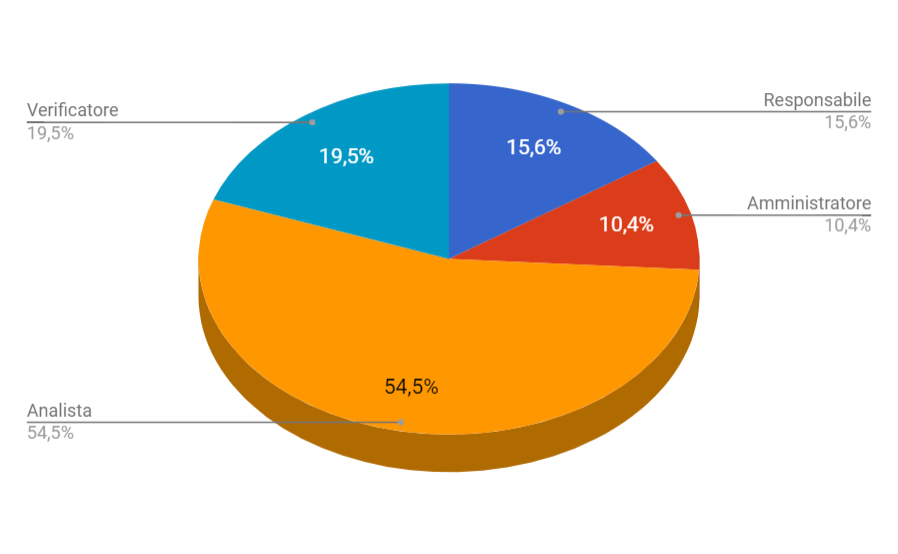
\includegraphics[width=11cm]{images/prospettoEconomico/progArch.png}
	\label{fig:foo}
	\caption{Grafico suddivisione dei ruoli del periodo di Progettazione architetturale}
\end{figure} 
\newpage
\section{Progettazione di dettaglio e codifica}
\subsection{Prospetto Orario}
Nel periodo di Progettazione di dettaglio e codifica la distribuzione oraria è la seguente:
\begin{center}
	\begin{table}[htbp]
		\centering
		\renewcommand\arraystretch{1.5}
		\begin{tabularx}{\textwidth}{p{4cm}|p{1cm}|p{1cm}|p{1cm}|p{1cm}|p{1cm}|p{1cm}|p{2cm}}
			\hline
			\textbf{Nome} & \textbf{Re} & \textbf{Ad} & \textbf{An} & \textbf{Pj} & \textbf{Pr} & \textbf{Ve} & \textbf{Totale} \\
			\hline
			\Davide & \ & 5 & \ & \ & 15 & 32 & \textbf{52} \\
			\hline
			\Elena & \ & \ & \ & 15 & 20 & 17 & \textbf{52} \\
			\hline
			\Gianluca & \ & \ & \ & 25 & 12 & 15 & \textbf{52} \\
			\hline
			\Mirco & \ & 6 & \ & 19 & 27 & \ & \textbf{52} \\
			\hline
			\Parwinder & 6 & \ & \ & 10 & 26 & 10 & \textbf{52} \\
			\hline
			\Riccardo & 8 & \ & \ & 25 & 19 & \ & \textbf{52} \\
			\hline
			\Valentina & \ & 8 & \ & 30 & 14 & \ & \textbf{52} \\
			\hline
		\end{tabularx}
	\caption{Distribuzione oraria del periodo di Progettazione in dettaglio e codifica}
	\label{my-label}
	\end{table} 	
\end{center}
Il seguente grafico dà una rappresentazione visiva della suddivisione oraria:
\begin{figure}[h]
	\centering
	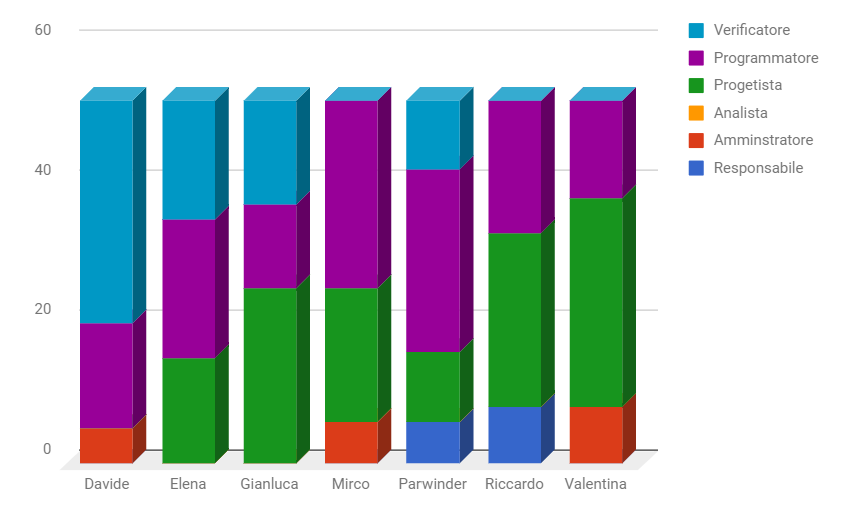
\includegraphics[width=10.5cm]{images/prospettoOrario/progCod.png}
	\label{fig:foo}
	\caption{Grafico suddivisione oraria del periodo di Progettazione di dettaglio e codifica}
\end{figure} 
\newpage
\subsection{Prospetto Economico}
Nel periodo di Progettazione di dettaglio e codifica la distribuzione delle ore tra i differenti ruoli è la seguente:\begin{center}
\begin{table}[htbp]
	\centering
	\renewcommand\arraystretch{1.5}
	\begin{tabularx}{\textwidth}{p{5cm}|p{4cm}|p{4cm}}
		\hline
		\textbf{Ruolo} & \textbf{Ore} & \textbf{Costo in \euro} \\
		\hline
		Responsabile & 14 & 420,00 \\
		\hline
		Amministratore & 19 & 380,00 \\
		\hline
		Analista & \ & \ \\
		\hline
		Progettista & 124 & 2.728,00 \\
		\hline
		Programmatore & 133 & 1995,00 \\
		\hline
		Verificatore & 74 & 1110,00 \\
		\hline
		\textbf{Totale} & \textbf{364} & \textbf{6633,00}\\
		\hline
	\end{tabularx}
	\caption{Prospetto economico del periodo di Progettazione in dettaglio e codifica}
	\label{my-label}
\end{table} 
\end{center}
Il seguente grafico dà una rappresentazione visiva della distribuzione dei ruoli:
\begin{figure}[h]
	\centering
	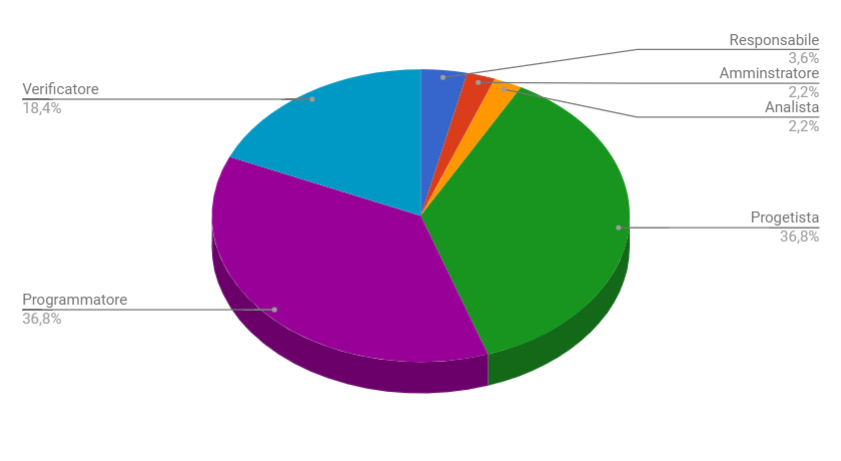
\includegraphics[width=12.5cm]{images/prospettoEconomico/progCod.png}
	\label{fig:foo}
	\caption{Grafico suddivisione dei ruoli del periodo di Progettazione di dettaglio e codifica}
\end{figure} 
\clearpage

\section{Validazione e collaudo}
\subsection{Prospetto Orario}
Nel periodo di Validazione e collaudo la distribuzione oraria è la seguente:
\begin{center}
	\begin{table}[htbp]
		\centering
		\renewcommand\arraystretch{1.5}
		\begin{tabularx}{\textwidth}{p{4cm}|p{1cm}|p{1cm}|p{1cm}|p{1cm}|p{1cm}|p{1cm}|p{2cm}}
			\hline
			\textbf{Nome} & \textbf{Re} & \textbf{Ad} & \textbf{An} & \textbf{Pj} & \textbf{Pr} & \textbf{Ve} & \textbf{Totale} \\
			\hline
			\Davide & \ & 8 & \ & 6 & \ & 6 & \textbf{20} \\
			\hline
			\Elena & \ & 8 & \ & \ & 6 & 6 & \textbf{20} \\
			\hline
			\Gianluca & 4 & \ & \ & 8 & \ & 8 & \textbf{20} \\
			\hline
			\Mirco & 6 & \ & \ & \ & \ & 14 & \textbf{20} \\
			\hline
			\Parwinder & \ & 7 & \ & \ & 6 & 7 & \textbf{20} \\
			\hline
			\Riccardo & \ & \ & \ & 8 & \ & 12 & \textbf{20} \\
			\hline
			\Valentina & \ & 4 & \ & 6 & 10 & \ & \textbf{20} \\
			\hline
		\end{tabularx}
	\caption{Distribuzione oraria del periodo di Verifica e collaudo}
	\label{my-label}
	\end{table} 	
\end{center}
Il seguente grafico dà una rappresentazione visiva della suddivisione oraria:
\begin{figure}[h]
	\centering
	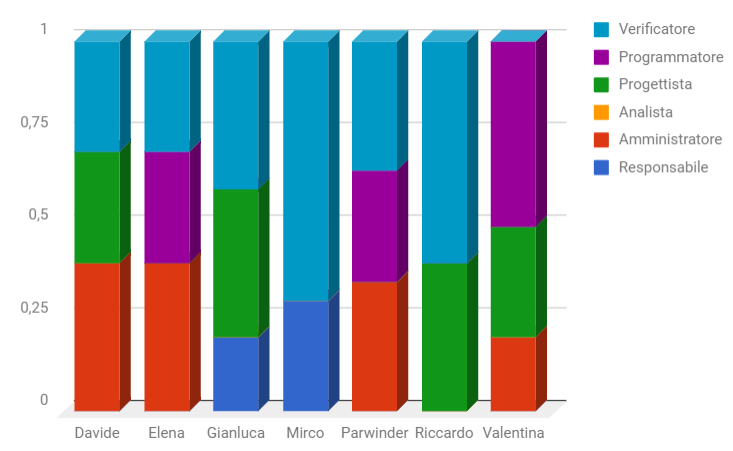
\includegraphics[width=10.5cm]{images/prospettoOrario/valCol.png}
	\label{fig:foo}
	\caption{Grafico suddivisione oraria del periodo di Validazione e collaudo}
\end{figure} 
\newpage
\subsection{Prospetto Economico}
Nel periodo di Validazione e collaudo la distribuzione delle ore tra i differenti ruoli è la seguente:
\begin{center}
	\begin{table}[htbp]
		\centering
		\renewcommand\arraystretch{1.5}
		\begin{tabularx}{\textwidth}{p{5cm}|p{4cm}|p{4cm}}
			\hline
			\textbf{Ruolo} & \textbf{Ore} & \textbf{Costo in \euro} \\
			\hline
			Responsabile & 10 & 300,00 \\
			\hline
			Amministratore & 27 & 540,00 \\
			\hline
			Analista & \ & \ \\
			\hline
			Progettista & 28 & 616,00 \\
			\hline
			Programmatore & 22 & 330,00 \\
			\hline
			Verificatore & 53 & 795,00 \\
			\hline
			\textbf{Totale} & \textbf{140} & \textbf{2581,00}\\
			\hline
		\end{tabularx}
	\caption{Prospetto economico del periodo di Verifica e collaudo}
	\label{my-label}
	\end{table} 
\end{center}
Il seguente grafico dà una rappresentazione visiva della distribuzione dei ruoli:
\begin{figure}[h]
	\centering
	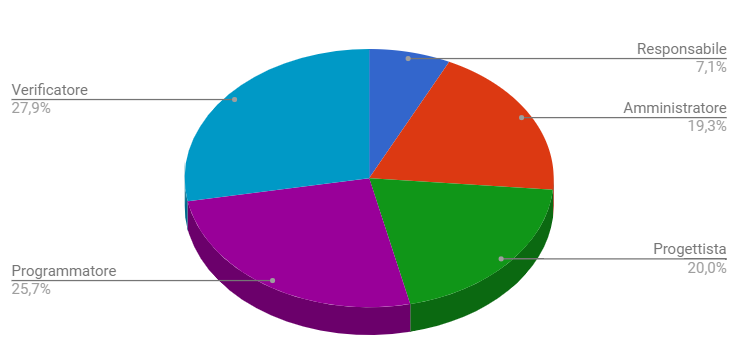
\includegraphics[width=12.5cm]{images/prospettoEconomico/valCol.png}
	\label{fig:foo}
	\caption{Grafico suddivisione dei ruoli del periodo di Validazione e collaudo}
\end{figure} 
\clearpage
\section{Totale ore rendicontate}
\subsection{Totale suddivisione ore rendicontate}
Di seguito sono riportate il totale delle sole ore rendicontate nel preventivo a carico del committente:
\begin{center}
	\begin{table}[htbp]
		\centering
		\renewcommand\arraystretch{1.5}
		\begin{tabularx}{\textwidth}{p{4cm}|p{1cm}|p{1cm}|p{1cm}|p{1cm}|p{1cm}|p{1cm}|p{2cm}}
			\hline
			\textbf{Nome} & \textbf{Re} & \textbf{Ad} & \textbf{An} & \textbf{Pj} & \textbf{Pr} & \textbf{Ve} & \textbf{Totale} \\
			\hline
			\Davide & 4 & 13 & 10 & 18 & 15 & 42 & \textbf{102} \\
			\hline
			\Elena & \ & 8 & \ & 35 & 26 & 33 & \textbf{102} \\
			\hline
			\Gianluca & 4 & 5 & \ & 48 & 12 & 33 & \textbf{102} \\
			\hline
			\Mirco & 10 & 6 & \ & 39 & 27 & 20 & \textbf{102} \\
			\hline
			\Parwinder & 6 & 7 & \ & 25 & 32 & 32 & \textbf{102} \\
			\hline
			\Riccardo & 8 & 5 & \ & 53 & 19 & 17 & \textbf{102} \\
			\hline
			\Valentina & 2 & 12 & 10 & 46 & 24 & 8 & \textbf{102} \\
			\hline
		\end{tabularx}
	\caption{Distribuzione oraria totale delle ore rendicontate}
	\label{my-label}
	\end{table}
	
\end{center}
Il seguente grafico dà una rappresentazione visiva della suddivisione oraria:\\
\begin{figure}[h]
	\centering
	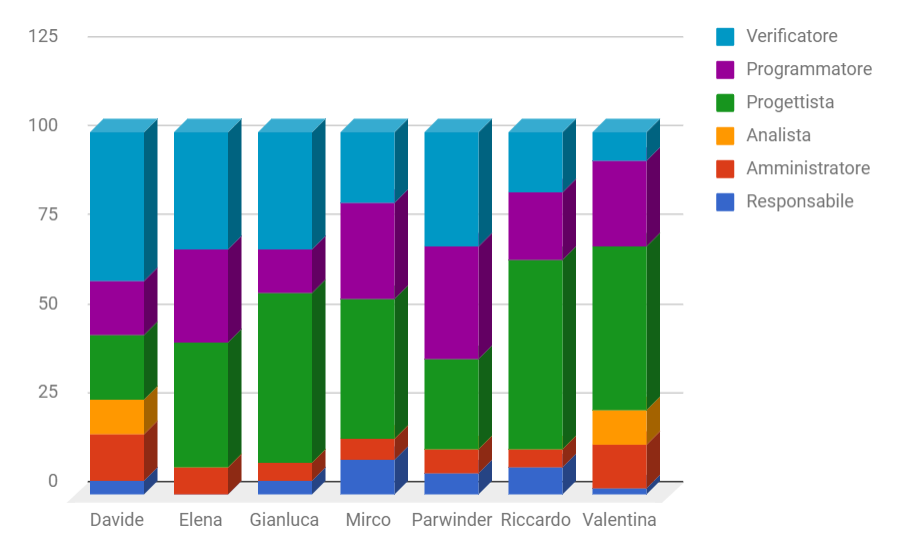
\includegraphics[width=10cm]{images/prospettoOrario/totRen.png}
	\label{fig:foo}
	\caption{Grafico suddivisione oraria totale delle ore rendicontate}
\end{figure} 
\clearpage
\subsection{Totale del prospetto economico rendicontato}
Di seguite è riportato il totale delle ore dei diversi ruoli del progetto contando solo le ore rendicontate nel preventivo a carico del committente cioè dei periodi di Progettazione architetturale, Progettazione di dettaglio e codifica e il periodo di Validazione e collaudo:
\begin{center}
	\begin{table}[htbp]
		\centering
		\renewcommand\arraystretch{1.5}
		\begin{tabularx}{\textwidth}{p{5cm}|p{4cm}|p{4cm}}
			\hline
			\textbf{Ruolo} & \textbf{Ore} & \textbf{Costo in \euro} \\
			\hline
			Responsabile & 34 & 1.020,00 \\
			\hline
			Amministratore & 56 & 1.120,00 \\
			\hline
			Analista & 20 & 500,00 \\
			\hline
			Progettista & 264 & 5.808,00 \\
			\hline
			Programmatore & 155 & 2.325,00 \\
			\hline
			Verificatore & 185 & 2.775,00 \\
			\hline
			\textbf{Totale} & \textbf{910} & \textbf{13.548,00}\\
			\hline
		\end{tabularx}
	\caption{Prospetto economico totale delle ore rendicontate}
	\label{my-label}
	\end{table} 
\end{center}
Il seguente grafico dà una rappresentazione visiva della distribuzione dei ruoli:
\begin{figure}[h]
	\centering
	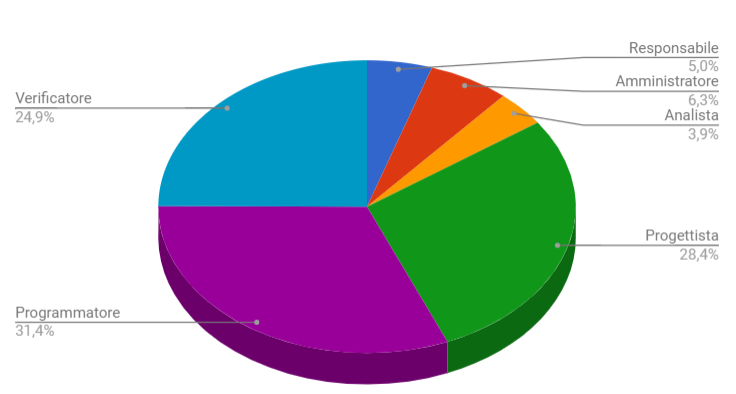
\includegraphics[width=10.5cm]{images/prospettoEconomico/totRen.png}
	\label{fig:foo}
	\caption{Grafico suddivisione dei ruoli totale delle ore rendicontate}
\end{figure} 
\clearpage
\section{Totale ore con investimento}
\subsection{Totale suddivisione ore con investimento}
Di seguito sono riportate il totale delle ore del progetto contando le ore di investimento e delle ore rendicontate nel preventivo a carico del committente:
\begin{center}
\begin{table}[htbp]
	\centering
	\renewcommand\arraystretch{1.5}
	\begin{tabularx}{\textwidth}{p{4cm}|p{1cm}|p{1cm}|p{1cm}|p{1cm}|p{1cm}|p{1cm}|p{2cm}}
		\hline
		\textbf{Nome} & \textbf{Re} & \textbf{Ad} & \textbf{An} & \textbf{Pj} & \textbf{Pr} & \textbf{Ve} & \textbf{Totale} \\
		\hline
		\Davide & 4 & 24 & 21 & 18 & 15 & 48 & \textbf{130} \\
		\hline
		\Elena & 8 & 12 & 16 & 35 & 26 & 33 & \textbf{130} \\
		\hline
		\Gianluca & 8 & 5 & 18 & 48 & 12 & 39 & \textbf{130} \\
		\hline
		\Mirco & 10 & 10 & 20 & 39 & 27 & 24 & \textbf{130} \\
		\hline
		\Parwinder & 14 & 11 & 14 & 25 & 32 & 34 & \textbf{130} \\
		\hline
		\Riccardo & 12 & 7 & 12 & 53 & 19 & 27 & \textbf{130} \\
		\hline
		\Valentina & 6 & 12 & 20 & 46 & 24 & 22 & \textbf{130} \\
		\hline
	\end{tabularx}
	\caption{Distribuzione oraria totale delle ore di investimento e rendicontate}
	\label{my-label}
\end{table}
\end{center}
Il seguente grafico dà una rappresentazione visiva della suddivisione oraria:
\begin{figure}[h]
	\centering
	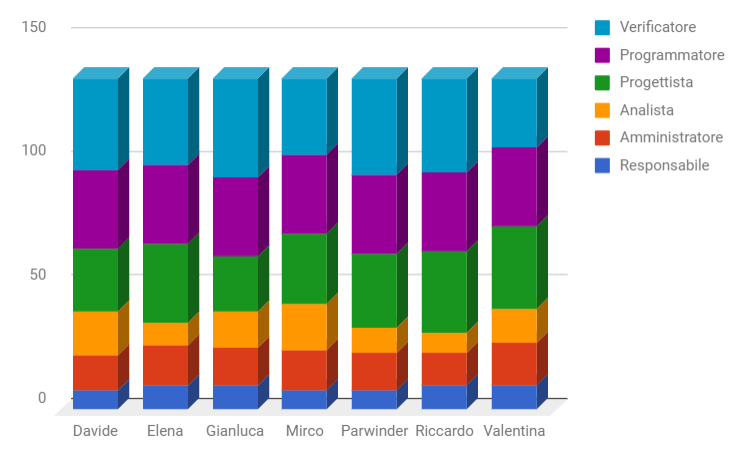
\includegraphics[width=10.5cm]{images/prospettoOrario/totale.png}
	\label{fig:foo}
	\caption{Grafico suddivisione oraria totale delle ore di investimento e rendicontate}
\end{figure} 
\clearpage
\subsection{Totale del prospetto economico con investimento}
Di seguito è riportato il totale delle ore dei diversi ruoli del progetto contando le ore di investimento e delle ore rendicontate nel preventivo a carico del committente:
\begin{center}
	\begin{table}[htbp]
		\centering
		\renewcommand\arraystretch{1.5}
		\begin{tabularx}{\textwidth}{p{5cm}|p{4cm}|p{4cm}}
			\hline
			\textbf{Ruolo} & \textbf{Ore} & \textbf{Costo in \euro} \\
			\hline
			Responsabile & 62 & 1.860,00 \\
			\hline
			Amministratore & 81 & 1.620,00 \\
			\hline
			Analista & 121 & 3.025 \\
			\hline
			Progettista & 264 & 5.808,00 \\
			\hline
			Programmatore & 155 & 2.325,00 \\
			\hline
			Verificatore & 227 & 3.405,00 \\
			\hline
			\textbf{Totale} & \textbf{910} & \textbf{18.043,00}\\
			\hline
		\end{tabularx}
	\caption{Prospetto economico totale delle ore di investimento e rendicontate}
	\label{my-label}
	\end{table} 
\end{center}
Il seguente grafico dà una rappresentazione visiva della distribuzione dei ruoli:
\begin{figure}[ht]
	\centering
	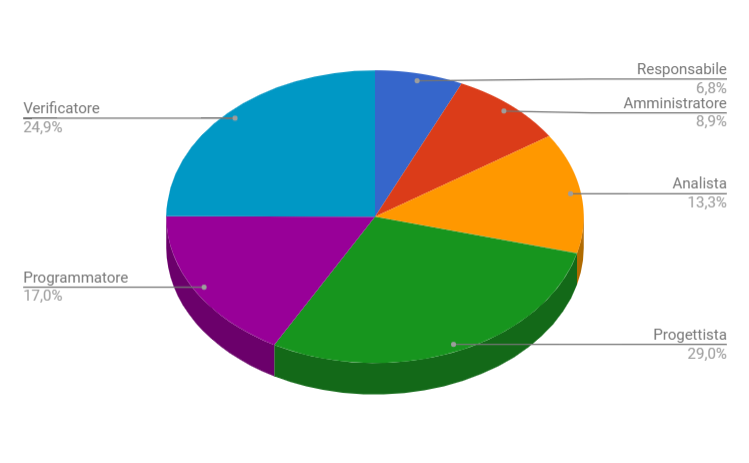
\includegraphics[width=10.5cm]{images/prospettoEconomico/totInv.png}
	\label{fig:foo}
	\caption{Grafico suddivisione totale dei ruoli delle ore di investimento e rendicontate}
\end{figure} 

\end{document}